\chapter{Configuring Eclipse and NetBeans for Java/Mongo development}

\begin{itemize}
\item Go to \url{http://central.maven.org/maven2/org/mongodb/mongo-java-driver/} and choose the right version.
\item In Eclipse, just start a new project \textbf{File - New - Java Project}
\item Right-click in \textbf{Properties} and then \textbf{Java Build Path - Libraries - Add External JARs} 

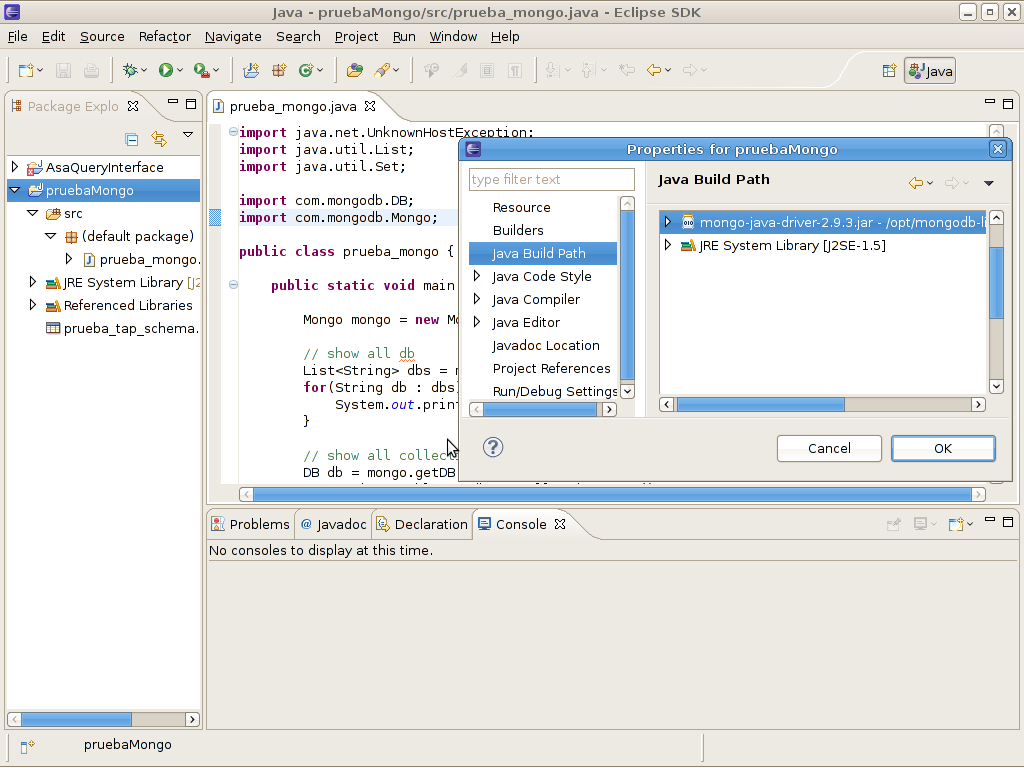
\includegraphics[height=8cm]{images/mongo_eclipse.png}

\item Import MongoDB methods, classed and interfaces as needed.
\item In NetBeans, start a new project \textbf{File - New Project - Java Application}
\item Right-click in \textbf{Libraries} and then \textbf{Add JAR/Folder} 

 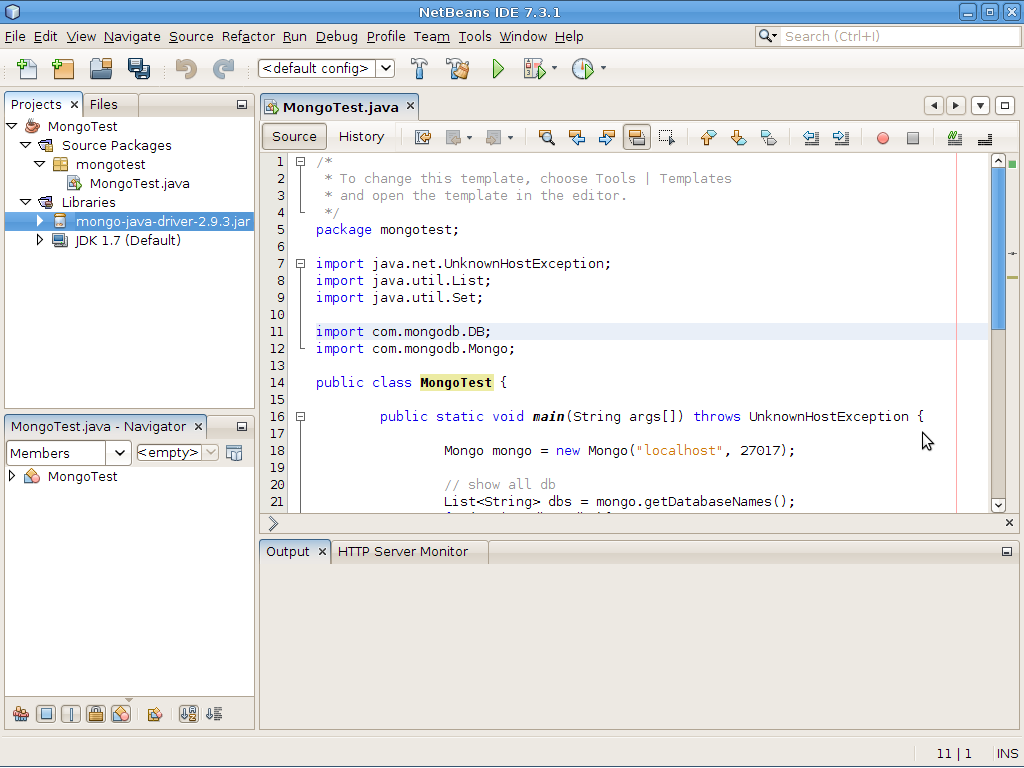
\includegraphics[height=8cm]{images/mongo_netbeans.png}

\item Import MongoDB methods, classed and interfaces as needed.
\end{itemize}
